Before performing the actual learning and prediction tasks, this chapter explores the data
in order to understand the statistics of the different features.

\subsection{Features}

After pre processing the data the data set to be explorted is describe in the following table:

\begin{table}[ht!]
\begin{center}
\begin{tabular}{llllrr}
\toprule
Field &  Description & Type &\\
\midrule
     p\_da & dialog act & categorical\\
     da & current dialog act & categorical \\
     secs & length of the current dialog act in seconds & numeric \\
     words & length of the current dialog act in words & numeric \\
     tsec & length of the current turn in words & numeric \\
     precent\_secs\_sofar  & length of the current turn in words & numeric \\
     precent\_words\_sofar & length of the current turn in words & numeric \\
     time\_control & length of the current turn in words & numeric \\
     words\_control & length of the current turn in words & numeric \\
     tchange & was a turn change after this dialog act & binary \\
\bottomrule
\end{tabular}
\end{center}
\caption{Precision, recall and F1 results }
\end{table}


\subsubsection{Dialog Acts}

The following chart show the count for each dialog act

 \begin{figure}
 \centering
 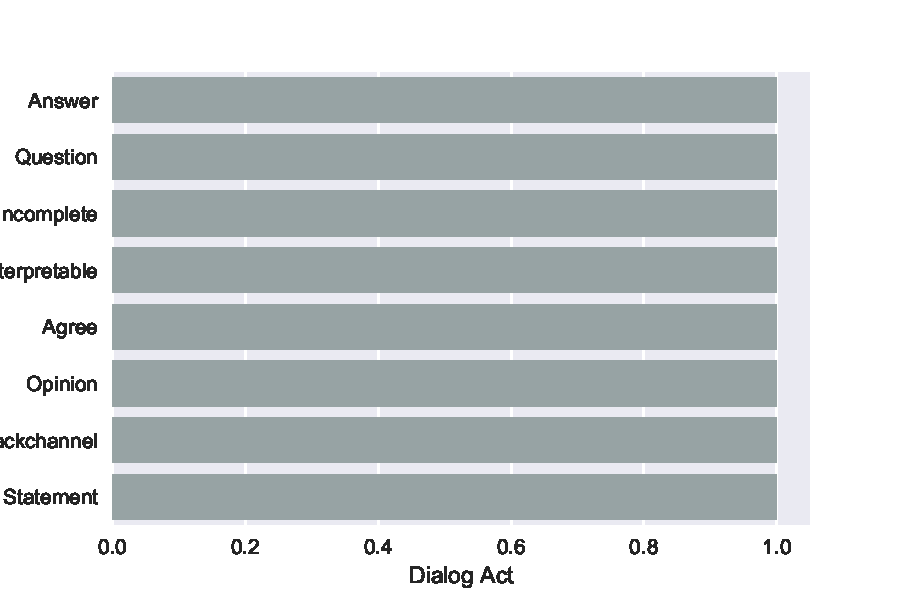
\includegraphics[width=0.5\textwidth]{../scikitlearn/figures/countplot_da_name_count.pdf}
 \caption{Dialog act size\label{overflow}}
 \end{figure}

We can further divide the measurements by creating the histogram for each dialog act. As expected most dialog act are short in length, however most observation are long tailed.


 \begin{figure}
 \centering
 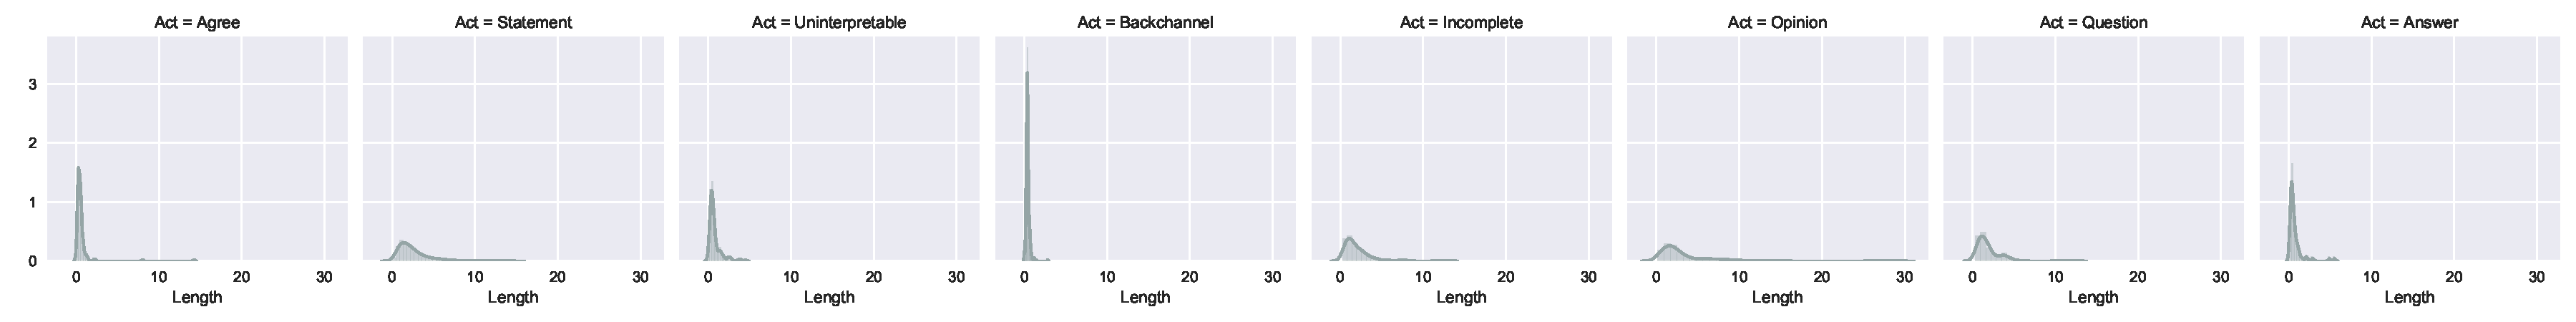
\includegraphics[width=\textwidth]{../scikitlearn/figures/grid_secs_by_da_name.pdf}
 \caption{Dialog act length in words \label{overflow}}
 \end{figure}
 
 We can further investigate if there the difference distribution when a dialog act lead to a turn change
 and the case where is does not. We can observe that the length distribution is the same, however when the 
 dialog act lead to a turn some question dialog acts are longer. 

\begin{figure}
 \centering
 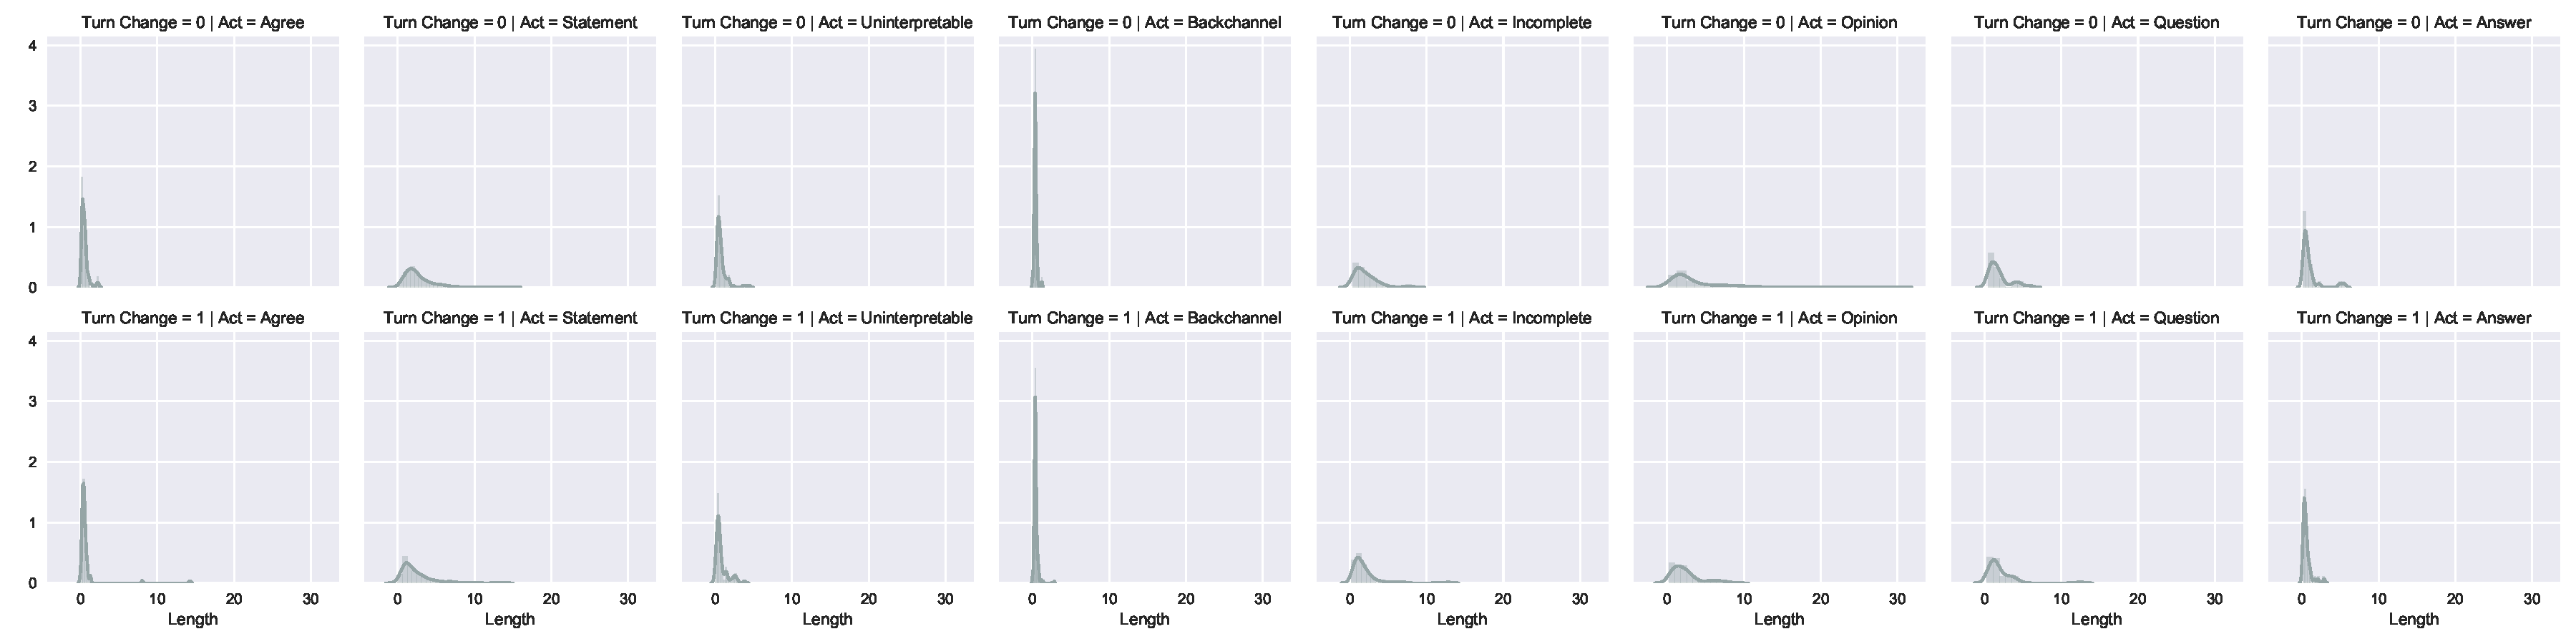
\includegraphics[width=\textwidth]{../scikitlearn/figures/grid_secs_by_da_name_by_tchange.pdf}
 \caption{Dialog act length in words conditioned on turn change\label{overflow}}
 \end{figure}
 
An interesting observation is measuring the probability that a dialog act will lead to turn change. 
The following chart shows that back channels and question will usually lead to turn change. 

\begin{figure}
\centering
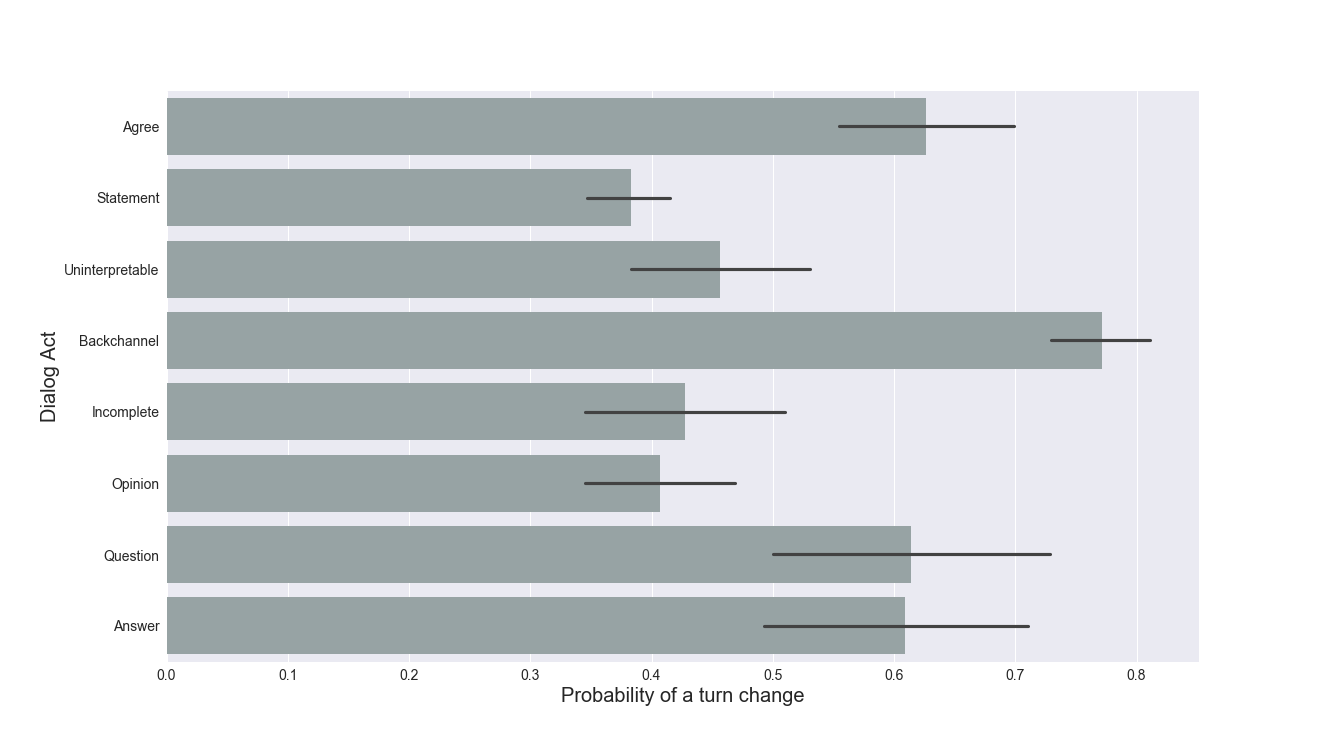
\includegraphics[width=\textwidth]{../scikitlearn/figures/barplot_da_prob_to_tchange.png}
\caption{Dialog act probability of turn change\label{overflow}}
\end{figure}


\subsection{Relative Turn Length}

The following chart shows distribution of the relative turn length for each dialog act. We can observe
that <TBD>

\begin{figure}
\centering
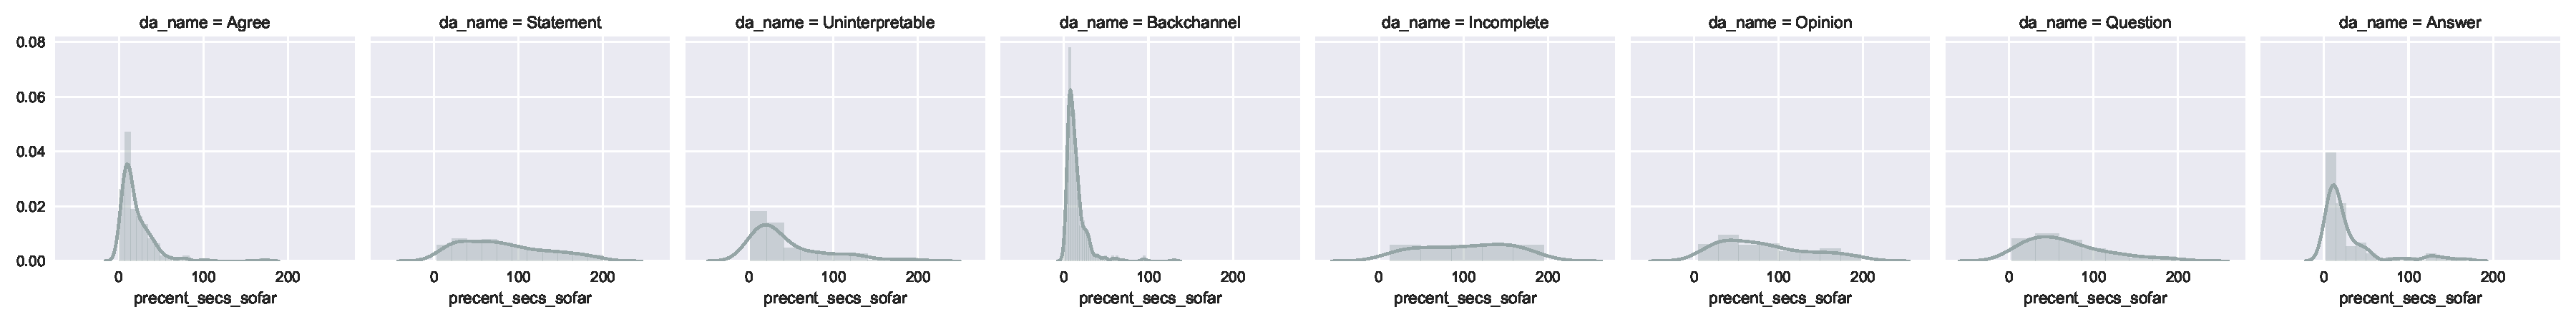
\includegraphics[width=\textwidth]{../scikitlearn/figures/grid_precent_secs_sofar_by_da_name.pdf}
\caption{Relative turn length for each dialog act\label{overflow}}
\end{figure}
 

\subsection{Relative Floor Control}

The following chart shows distribution of floor control or each dialog act conditioned on a turn change. We can observe that regradless of the dialog act, most distributions are normal with mean of 50\%

\begin{figure}
\centering
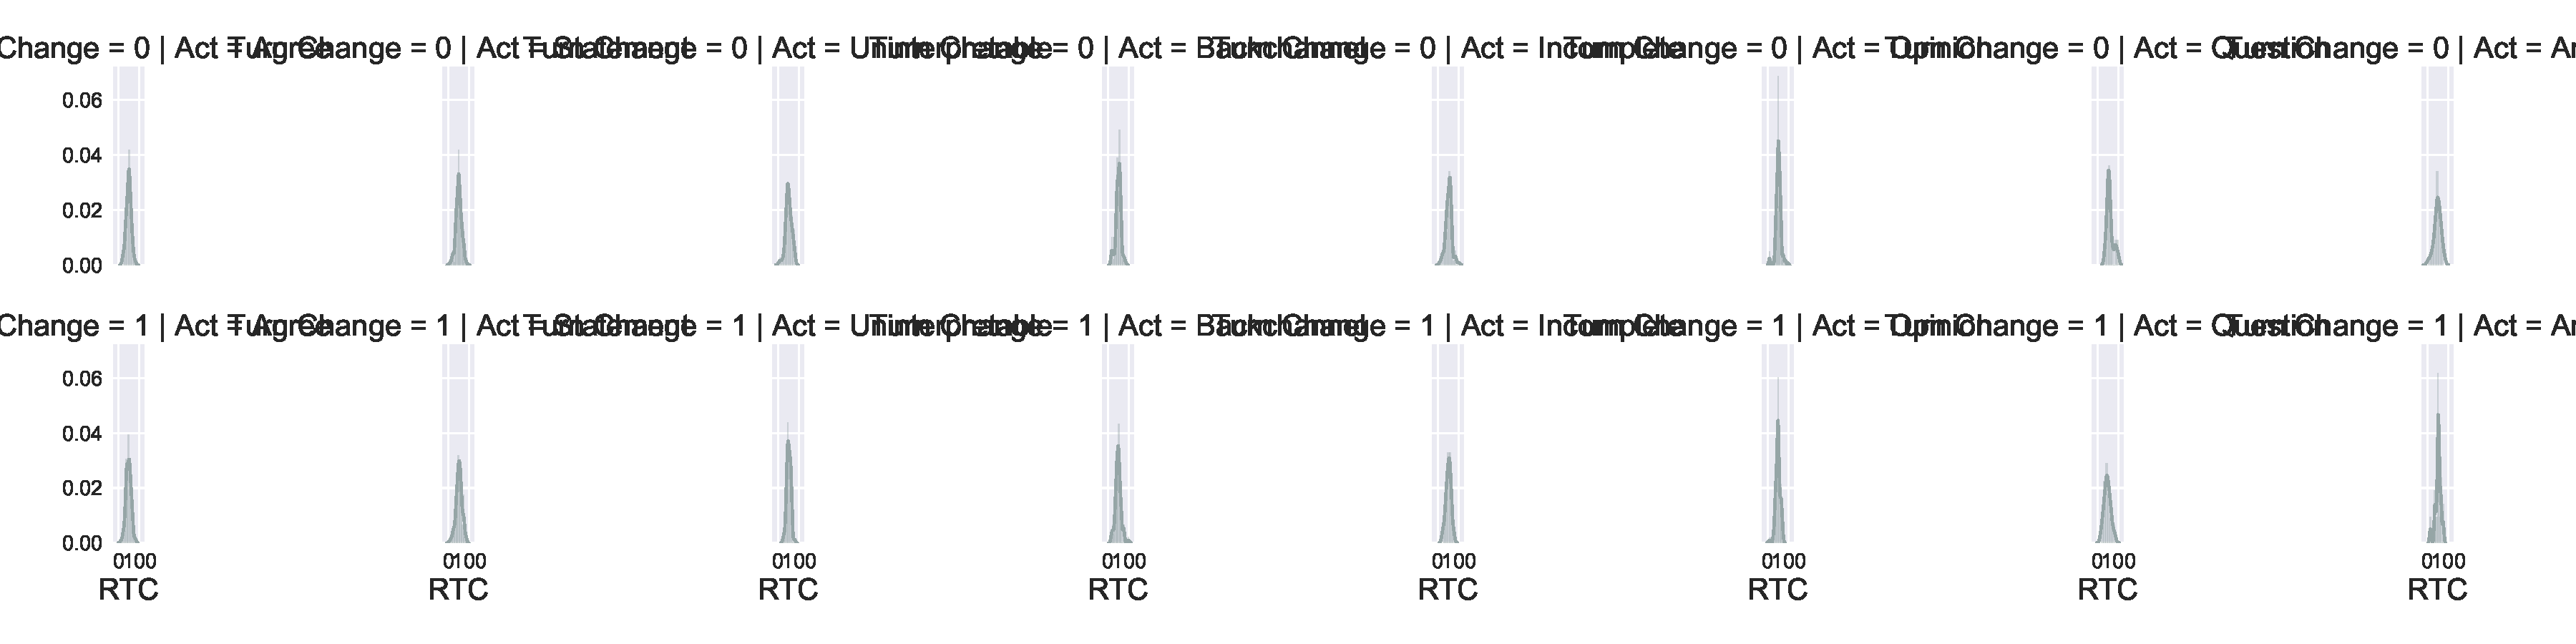
\includegraphics[width=\textwidth]{../scikitlearn/figures/grid_timecontrol_by_da_name_by_tchange.pdf}
\caption{Relative flow control conditioned on turn change\label{overflow}}
\end{figure}


